\documentclass[pdf]{beamer}
%\beamertemplateshadingbackground{red!10}{blue!10}

\usepackage{multirow}
%\usepackage{beamerthemeshadow}

\usepackage[T1]{fontenc}
\usepackage[french]{babel}
\usepackage{beamerthemeMalmoe}
%\usetheme{Warsaw}
%\useoutertheme{infolines}
\usepackage[utf8]{inputenc}
\usepackage{xspace}

\usepackage{alltt}


\newcommand{\softName}{uima@rcln\xspace}
\newcommand{\utilsModule}{{\em lipn-nlptools-utils}\xspace}
\newcommand{\uimaModule}{{\em lipn-uima-core}\xspace}

%\usepackage[french]{algo_erwan}
\beamertemplatetransparentcovereddynamic

\beamerboxesdeclarecolorscheme{mabox}{blue!60!averagebackgroundcolor}{blue!8!averagebackgroundcolor}


\setbeamertemplate{footline}{%
 \begin{beamercolorbox}[colsep=1.5pt]{upper separation line foot}
 \end{beamercolorbox}
 \begin{beamercolorbox}[ht=2.5ex,dp=1.125ex,%
   leftskip=.3cm,rightskip=.3cm plus1fil]{title in head/foot}%
   \leavevmode{\usebeamerfont{title in head/foot}\insertshorttitle\ (\insertshortauthor)}%
%   \leavevmode{\usebeamerfont{title in head/foot}\insertshorttitle}%
   \hfill%
   {\usebeamerfont{title in head/foot}\usebeamercolor[fg]{institute in head/foot}\insertframenumber/\inserttotalframenumber}%
 \end{beamercolorbox}%
 \begin{beamercolorbox}[colsep=1.5pt]{lower separation line foot}
 \end{beamercolorbox}
}
\setbeamertemplate{navigation symbols}{}

\newcommand{\todo}[1]{{\bf [TODO: #1]}}

\newcommand{\rien}[1]{}
\newcommand{\temp}[1]{{\bf [#1]}}
\newcommand{\colok}{Black}
\newcommand{\colno}{BrickRed}
\newcommand{\ccite}[1]{{\small #1}}
\newcommand{\noeud}{n\oe ud\xspace}
\newcommand{\noeuds}{n\oe uds\xspace}

\newcommand{\smallpar}[1]{{\footnotesize \it (#1)}}

\title{Introduction à la plateforme d'annotation \softName}


%\subtitle{}

\author{Erwan Moreau}

\date{14 octobre 2010}


\institute{
%Postdoc LIPN\\
Université Paris 13 \& UMR CNRS 7030\\
\url{erwan.moreau@lipn.univ-paris13.fr}
}

\begin{document}
\frame{
\titlepage
}

\section{Introduction}

\subsection{Présentation}

\frame{
\frametitle{Principaux objectifs (1)}

\begin{itemize}
\item Mise à jour / amélioration de ``l'utilisabilité'' des outils de la plateforme Ogmios/Alvis
\begin{itemize}
\item {\bf TreeTagger, YaTeA}
\item permettre utilisation en ``boîte noire''
\end{itemize}
\end{itemize}
\begin{itemize}
\item Jeter les bases d'une plateforme UIMA dédiée aux tâches étudiées par l'équipe (annotation sémantique)
\begin{itemize}
\item à long terme: améliorer la {\bf gestion/organisation des développements logiciels} de l'équipe
\item outils plus uniformes, compatibles, modulables, maintenace facilitée
\item {\bf évolutivité}
\end{itemize}
\end{itemize}
}


\frame{
\frametitle{Principaux objectifs (2)}

\begin{itemize}
\item Proposer une nouvelle approche dans la conception d'un {\em Type System}
\begin{itemize}
\item {\bf générique}: permettre/faciliter la composition de composants dans une chaîne
\begin{itemize}
\item transmission des données entre composants non homogènes
\end{itemize}
\item qui permet les {\bf annotations concurrentes}
\end{itemize}
\end{itemize}

Secondairement :
\begin{itemize}
\item Librairies ``utilitaires'' Java 

\item Possibilité de mise en place d'une politique de gestion logicielle
\begin{itemize}
\item ... si les intéressés le souhaitent bien sûr !
\end{itemize}
\end{itemize}
}

\frame{
\frametitle{UIMA en bref}

\begin{itemize}
\item un {\em Framework} pour ``encadrer'' l'analyse de grands volumes de données non structurées
\begin{itemize}
\item ``analyse'' $\approx$ découverte de connaissances ``utiles''
\item implémentation nettement orientée données textuelles
\end{itemize}
\item[$\rightarrow$] Ensemble d'{\bf outils} et (surtout) de {\bf conventions}
\begin{itemize}
\item But: partage, faciliter la communication inter-composants
\item Systèmes complexes avec composants indépendants mais composables
\item[$\Rightarrow$] Standardisation des composants + flexibilité
\end{itemize}
\item Implémentation Apache UIMA en {\bf Java}
\begin{itemize}
\item open-source, développement rapide
\end{itemize}
\end{itemize}
}



\frame{
\frametitle{Caractéristique: composants par encapsulation}


\begin{itemize}
\item Appel à un programme externe pour la réalisation de la tâche 
\item[$\rightarrow$] Avantage :  coût de développement moindre, outils connus
\item[$\rightarrow$] Inconvénients nombreux, non conforme à philosophie UIMA 
\begin{itemize}
\item portabilité $\searrow$ 
\item failles potentielles (entrées/sorties, gestion d'erreurs, multi-threading)
\item rupture du contrôle UIMA sur les composants
\begin{itemize}
\item conséquences sur chaîne complexe
\end{itemize}
\item perte d'efficacité temps/espace
\end{itemize}
\end{itemize}

\begin{itemize}
\item Gestion de ces problèmes
\begin{itemize}
\item Librairie d'appel ``protégé'' à un programme extérieur
\begin{itemize}
\item possibilité de lire/écrire à la volée
\end{itemize}
\item Librairie de (ré)-alignement, conversion entre formats
%\begin{itemize}
%\item modulable et paramétrable
%\end{itemize}
\end{itemize}
\end{itemize}
}


%\subsection{Contexte}

\frame{
\frametitle{Contexte}

\begin{itemize}
\item Projet Quaero
\begin{itemize}
\item WP 3.4 ``Développement d'une nouvelle plateforme d'annotation''
\end{itemize}
\item Casting :
\begin{itemize}
\item Maître d'\oe uvre : Laurent Audibert
\item Travail préliminaire par Sondes Bannour
\item Aide du LINA (Univ Nantes), notamment Fabien Poulard
\end{itemize}
\item Prototype quasi-``version beta'' {\small (phase tests utilisateurs)}
\begin{itemize}
\item Composants principaux terminés
\item Ajout des dernières fonctionnalités 
\item Documentation en cours de rédaction
\item {\em Release} version stable très bientôt
\end{itemize}
\end{itemize}
}


\frame[plain]{
%\frametitle{Une page de publicité}

\noindent\begin{center}
\noindent\scalebox{.37}[.37]{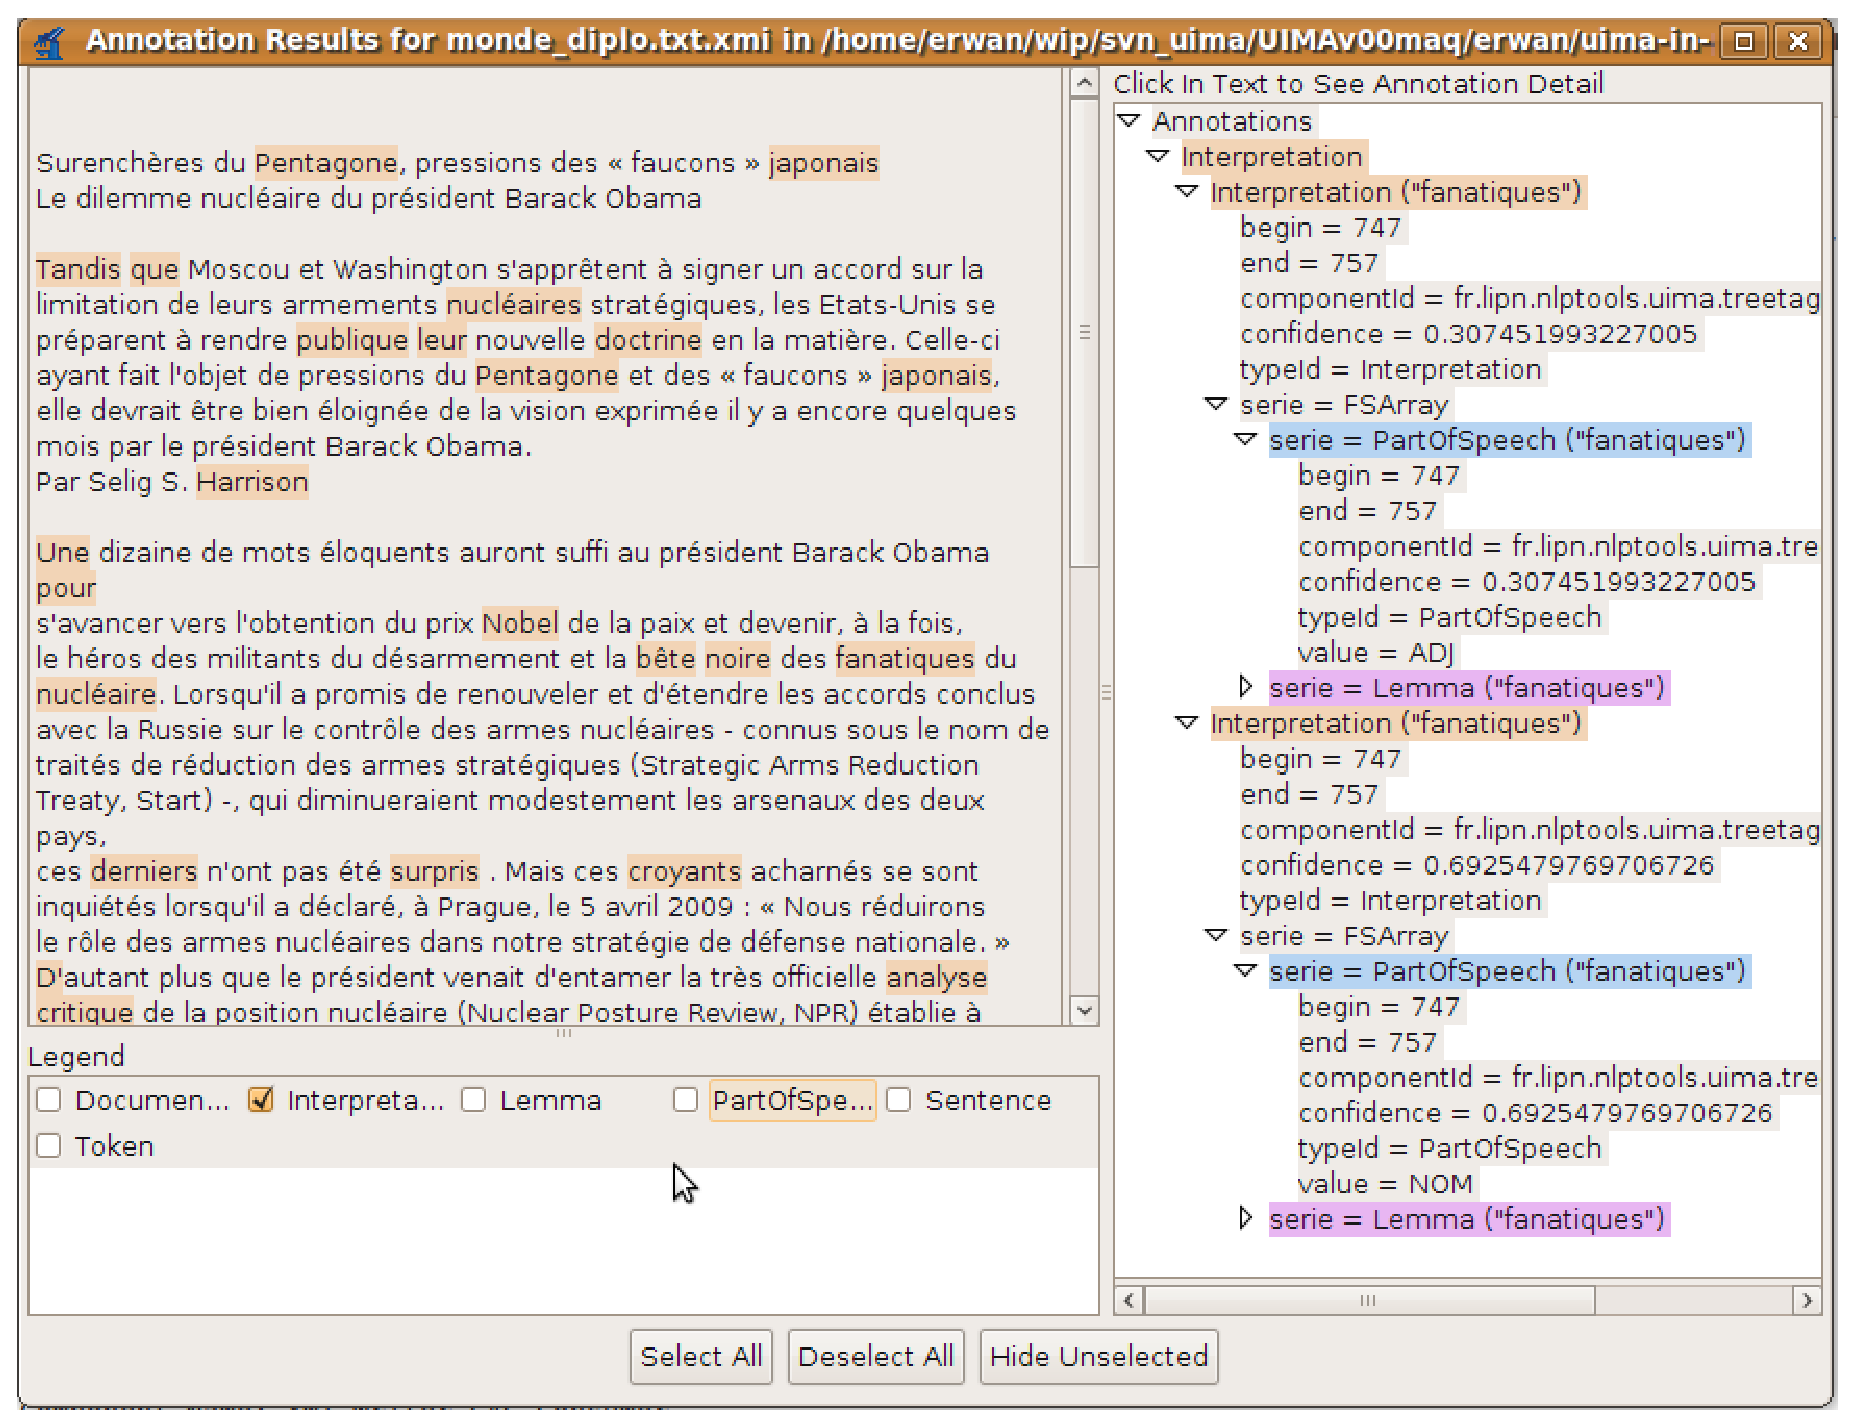
\includegraphics{capture_viewer_expl_interpretations.eps}}
\end{center}

}

\frame{
\frametitle{Plan}
\tableofcontents[hideallsubsections]

}



\section{Le framework UIMA}


\frame{

\tableofcontents[sectionstyle=show/hide,hideothersubsections]

}


\subsection{Présentation, objectifs} % communauté

\frame{
\frametitle{UIMA: Introduction}
\begin{itemize}
\item Unstructured Information Management Applications:
\begin{itemize}
\item {\bf Spécification} définie par l'OASIS {\small (Organization for the Advancement of Structured Information Standards)}
\item {\bf Implémentation} initiée par IBM, reprise par Apache (2006)
\end{itemize}

\item But : encourager l'{\bf interopérabilité entre composants}
\begin{itemize}
\item {\em Représentation des données,} indépendance artefact / méta-données
\item {\em Modélisation/échanges de données} indépendants de la plateforme, forme ``programmable''
\item {\em Découverte, ré-utilisation et composition} de composants indépendants
\item {\em Interopérabilité au niveau services}
\end{itemize}
\end{itemize}
}

\frame{
\frametitle{Apache UIMA}

\begin{itemize}
\item Une implémentation {\bf Java} de la spécification UIMA OASIS
\item Un {\em framework} + un {\em SDK}:
\begin{itemize}
\item SDK : ensemble d'outils pour construire des composants UIMA via API
\item framework : librairies suffisantes pour déployer des composants
\end{itemize}
\item Open-source
\item Un projet Apache dynamique:
\begin{itemize}
\item Version 2.3 $\approx$ Janvier 2010, prochaine version bientôt
\item Apache ``top-level project'' depuis Mai 2010
\item Communauté d'utilisateurs grandissante (?)
\item Liste(s) d'utilisateurs active(s)
\end{itemize}
\end{itemize}

}

\subsection{Concepts généraux}

\frame{
\frametitle{Principe}
\begin{itemize}
\item Chaîne de traitement composée de:
\begin{itemize}
\item un {\em Collection Reader}, qui lit le(s) document(s)
\item une séquence d'{\em Annotator Engine (AE)}, procédant chacun à une tâche donnée
\item un/plusieurs AEs qui ``consomment'' le résultat {\footnotesize (ex- {\em CAS Consumers})}
\end{itemize}
\item Le CAS {\em (Common Analysis Structure)} contient :
\begin{itemize}
\item le document de départ (String)
\item les annotations (méta-données) ajoutées par les composants
\item le {\em Type System} 
\begin{itemize}
\item typologie pour la représentation des méta-données
\end{itemize}
\end{itemize}
\item Gestion du processus par le framework via un {\em Collection Processing Engine (CPE)} 
\begin{itemize}
\item Passage de paramètres, gestion d'erreurs, ``flot'' (e.g. parallélisation), ressources, log...
\end{itemize}
\end{itemize}
}

\frame{
\noindent\begin{center}
\noindent\hspace*{-.7cm}\scalebox{.35}[.4]{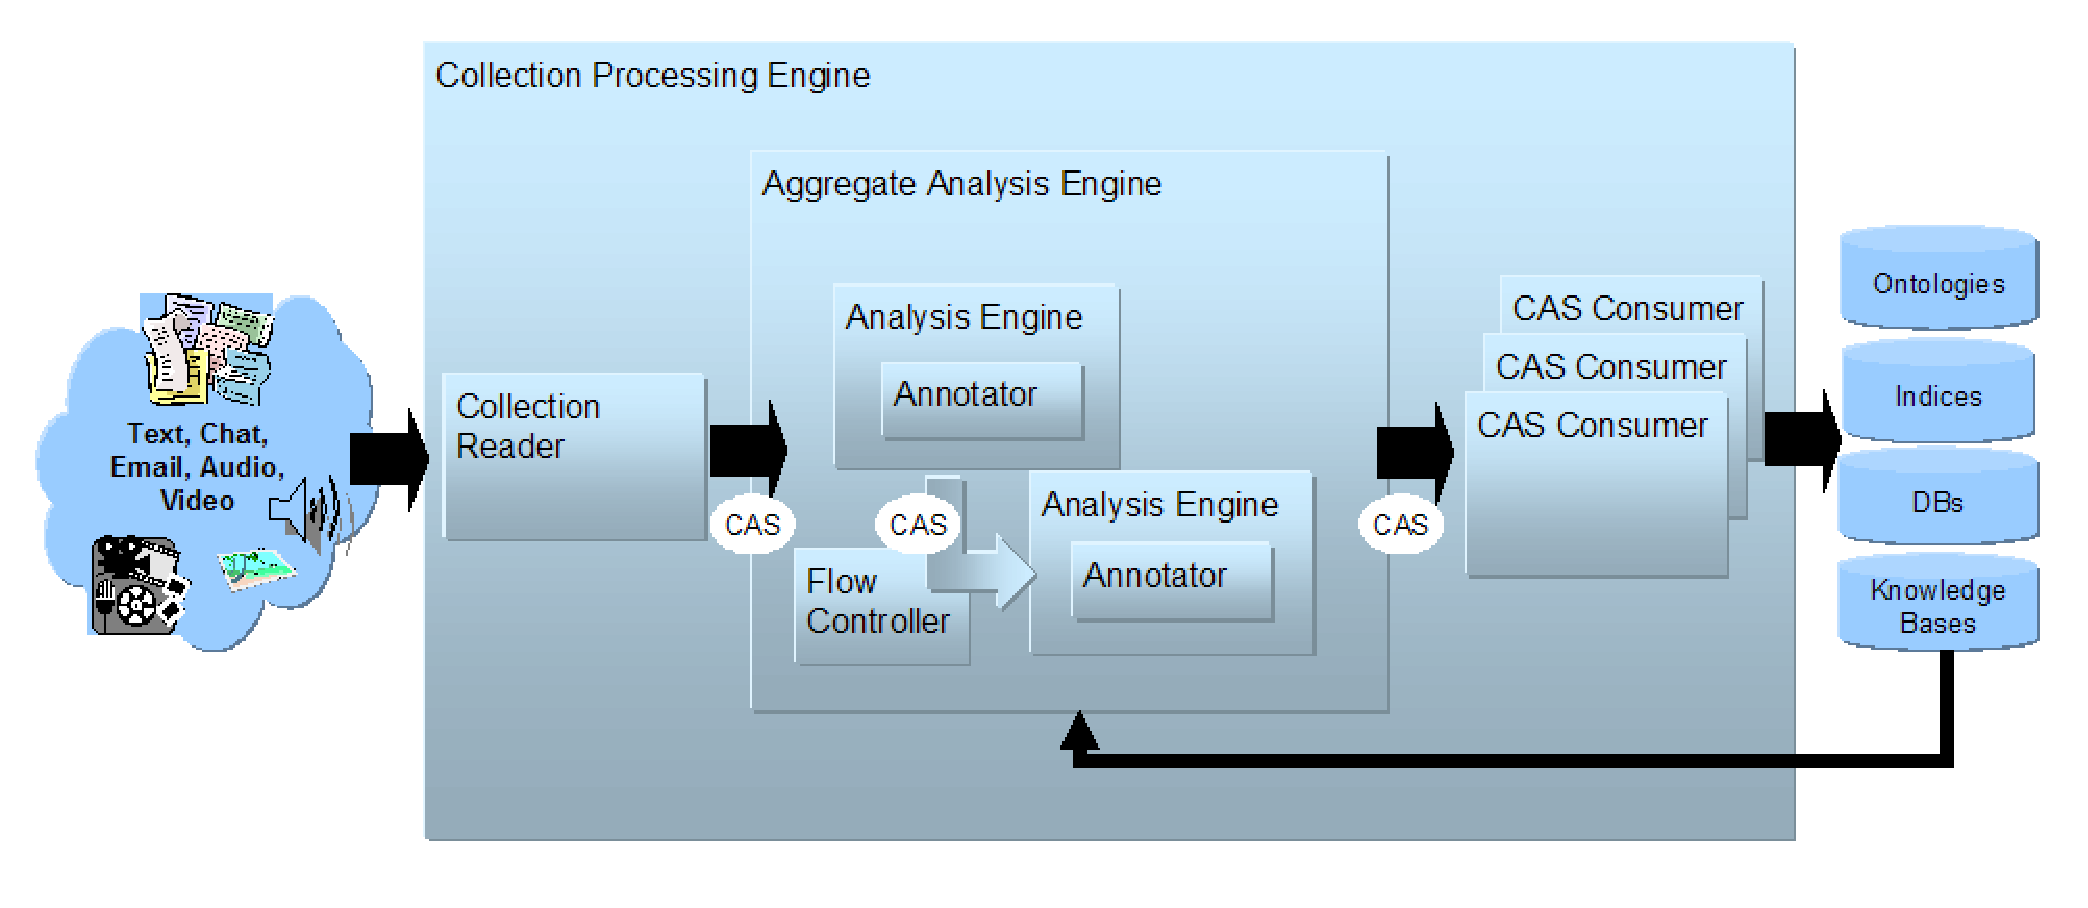
\includegraphics{uima_process.eps}}
\end{center}

}


\subsection{Type System}

\frame{
\frametitle{Représentation des méta-données: le Type System}

\begin{itemize}
\item Hiérarchie de types destinés à ``recevoir'' les annotations
\item un type peut comporter des attributs {\em (features)}
\begin{itemize}
\item ex: {\tt Individu} avec features {\tt nom}, {\tt prenom} de type {\tt String}
\item typage des features parmi types primitifs UIMA + tout type précédemment défini
\end{itemize}
\item Héritage classique
\begin{itemize}
\item ex: {\tt Chercheur} hérite de {\tt Individu}, feature {\tt h\_index} ajoutée.
\end{itemize}
\item Annotation (instance d'un type) accédée via objet Java 
\item[$\rightarrow$] {\bf MAIS} Type UIMA $\neq$ objet Java
\begin{itemize}
\item aucune méthode spécifique associée (accesseurs seuls)
\item interfaces/classes abstraites impossibles
\end{itemize}
\item Type standard {\tt org.apache.uima.jcas.tcas.Annotation}
\begin{itemize}
\item Features {begin}/{end} de type {int} = position dans le texte
\end{itemize}
\end{itemize}
}

\subsection{Annotateurs}

\frame{
\frametitle{Construire un annotateur}
\begin{itemize}
\item {\em Annotator Engine Descriptor} (fichier XML):
\begin{itemize}
\item Nom de la classe Java
\item Type System
\item Paramètres spécifiques
\begin{itemize}
\item Nommage, typage, description, affectation
\item NB: entrée/sortie = CAS
\end{itemize}
\item {\em Capabilities}: types nécessaire en entrée et fournis en sortie
\end{itemize}
\item Classe Java héritant de {\tt JCasAnnotator\_ImplBase}
\begin{itemize}
\item Méthode {\tt initialize(context)} : gestion des paramètres
\item Méthode {\tt process(aJCas)} : tâche proprement dite
\begin{itemize}
\item Accès au document : {\tt aJCas.getDocumentText()}
\item Accès aux annotations avec itérateurs : {\tt aJCas.getAnnotationIndex(myType).iterator()}
\item Écriture d'annotations : {\tt myAnnot = new MyType(aJCas)} ... {\tt myAnnot.addToIndexes()}
\end{itemize}
\end{itemize}
\end{itemize}
}

%\frame{
%\frametitle{Autres composants (aperçu)}

%\begin{itemize}
%\item {\em Collection Reader
%\end{itemize}
%}

\subsection{Outils standard UIMA}
\frame{
\frametitle{Outils (aperçu)}
\begin{itemize}
\item API pour gestion d'erreurs, {\em logging}, etc. 
\item Composant {\em Collection Reader} qui lit les fichiers $\rightarrow$ CAS
\item Composant {\em CAS consumer} qui écrit les données annotées en XML (format XMI)
\item Outils graphiques
\begin{itemize}
\item Costruction de descripteurs TS, AED (Eclipse)
\item Composition/configuration de CPE
\item Visualisation d'annotations
\end{itemize}
\item Nombreuses façons d'utiliser/lancer un traitement :
\begin{itemize}
\item CPE GUI (graphique)
\item script UIMA
\item programme Java
\end{itemize}
\end{itemize}
}


\subsection{Synthèse}


\frame{
\frametitle{Le framework UIMA : synthèse}

\begin{itemize}
\item Objectif essentiel : favoriser la {\bf compositionnalité} entre composants d'analyse
\item Moyen : {\bf standardisation} 
\begin{itemize}
\item de la représentation des données 
\item de ``l'interfaçage'' des composants (E/S, paramètres, etc.)
\end{itemize}
\item Difficultés :
\begin{itemize}
\item éviter de restreindre l'éventail des tâches représentables
\item rester $\approx$ simple à utiliser (développeur/utilisateur)
\item efficacité
\end{itemize}
\item Bénéfices secondaires :
\begin{itemize}
\item Librarie d'outils standard
\item Accès aux composants extérieurs existants
\end{itemize}
\end{itemize}
}

\frame{
\frametitle{Adopter UIMA ? (avis subjectif)}
\begin{itemize}
\item Inconvénients :
\begin{itemize}
\item Contraignant $\rightarrow$ construction + complexe, utilisation + laborieuse
\item Chronophage $\rightarrow$ apprentissage/adaptation, + de cas à gérer, - de marge de man\oe uvre
\item Rentabilité ? $\rightarrow$ moyen/long terme 
\begin{itemize}
\item Quand une ``masse critique'' de composants est disponible
\item Si ce standard reste dynamique
\end{itemize}
\end{itemize}
\item Avantages :
\begin{itemize}
\item Standardisation : modularité, flexibilité, communication
\item Favorise programmation ``propre'' 
\begin{itemize}
\item sinon, UIMA inutile !
\end{itemize}
\item[$\Rightarrow$] Bénéfice UIMA $\approx$ langage non structuré vs. structuré
\begin{itemize}
\item contraignant d'abord, rentable ensuite
\item + robuste, débuggage simplifié, maintenance facilité...
\end{itemize}
\end{itemize}
\end{itemize}
}


% pbms fréquents chemins, pratique nécessaire, apprentissage


\section{Approche \softName} 

\frame{

\tableofcontents[sectionstyle=show/hide,hideothersubsections]

}

\subsection{Objectifs} % plus précis

\frame{
\frametitle{Objectifs}

\begin{itemize}
\item Encapsuler les outils utilisés par l'équipe
\begin{itemize}
\item TagEN (entités nommées), TreeTagger (POS), YaTeA (termes) (+LIA)
\item en faciliter l'utilisation (robustesse, flexibilité)
\begin{itemize}
\item encodages, formats, problèmes d'alignement, etc.
\end{itemize}
\end{itemize}
\item Plateforme {\bf évolutive}
\begin{itemize}
\item proposant des outils de base, dont 
\begin{itemize}
\item composants et applications immédiates
\item ``utilitaires'' de base (pour utilisation actuelle et composants futurs)
\end{itemize}
\item sur laquelle des composants futurs {\em non prévisibles} peuvent s'intégrer
\begin{itemize}
\item éviter restrictions/contraintes $\rightarrow$ généricité
\end{itemize}
\item permettant l'usage d'annotations concurrentes
\end{itemize}
\end{itemize}
}
\frame{
\frametitle{Différents utilisateurs}

\begin{itemize}
\item {\bf Boîte noire.} lancer un CPE (chaîne de traitement) prédéfini, sans contrôle (ou peu) sur les paramètres
\item {\bf Outils non UIMA.} utiliser les librairies indépendantes
\item {\bf UIMA end-user} configurer une chaîne de traitement faite de composants UIMA $\rightarrow$ pré-requis UIMA léger
\item {\bf Programmeur UIMA} construire de nouveaux annotateurs basés sur le même ``c\oe ur'' $\rightarrow$ pré-requis UIMA+\softName 
\item {\bf Maintenance} construire/améliorer la base des composants \softName $\rightarrow$ pré-requis UIMA+\softName sérieux !
\end{itemize}
}

\frame{

\frametitle{Contraintes multiples}

\begin{itemize}
\item Niveau inférieur $\rightarrow$ outils encapsulés
\begin{itemize}
\item pas toujours bien spécifiés
\item pas toujours exempts de bugs
\item limitations intrinsèques
\item prévenir les problèmes liés à l'encapsulation
\end{itemize}
\item Niveau supérieur $\rightarrow$ différents  utilisateurs
\begin{itemize}
\item facilité d'utilisation utilisateur occasionel
\item liberté de paramétrage utilisateur avancé
\item API claire pour programmeur de composants
\item sans/peu contraintes pour composants futurs
\end{itemize}
\item Framework UIMA
\begin{itemize}
\item contraintes techniques/conceptuelles
\end{itemize}
\end{itemize}

}


\subsection{Composants par encapsulation}

\frame{
\frametitle{Appel externe à un outil : difficultés}

\begin{itemize}
\item {\bf Portabilité} abandonnée. 
\begin{itemize}
\item à souligner pour les composants concernés car rare
\end{itemize}
\item {\bf Sûreté} du procecssus UIMA diminuée
\begin{itemize}
\item rupture des mécanismes de contrôle (exceptions, log, ...)
\item failles potentielles du programme externe
\end{itemize}
\item {\bf Facilité d'emploi}  diminuée
\begin{itemize}
\item nécessité d'installer/localiser l'outil externe
\item parfois contraintes inattendues pour cadre UIMA
\item erreurs non filtrées du programme 
\end{itemize}
\item Transmission des {\bf entrées/sorties} 
\begin{itemize}
\item conversions de formats (erreurs, pertes)
\item erreurs ``physiques'' (échec, blocage)
\end{itemize}
\item {\bf Efficacité}
\begin{itemize}
\item perte en temps/espace pour transmission
\item surcharge mémoire (stockage en double)
\end{itemize}
\end{itemize}
}

\subsection{Choix / guidelines}

\frame{

\frametitle{Principe de précaution (bonnes pratiques)}

\begin{itemize}
\item Programmation modulaire
\begin{itemize}
\item Classes/packages dédiées à une tâche (ex: conversions)
\begin{itemize}
\item préférer classes Java officielles
\item ré-utilisabilité du code testé
\item gestion harmonisée des cas/paramètres
\item inconvénient : plus complexe
\item {\em bug-free} impossible $\rightarrow$ faciliter débuggage
\end{itemize}
\end{itemize}
\item Documentation claire et complète
\begin{itemize}
\item spécifications des composants, comportement particulier
\item choix d'implémentation
\end{itemize}
\item Respect des conventions le cas échéant
\begin{itemize}
\item faciliter reprise du code
\item ex: nommage de packages/classes, langue, etc.
\end{itemize}
\end{itemize}
}

\subsection{Type System}

\frame{
\frametitle{Orientation du Type System} % intérêts, expls
\begin{itemize}
\item 2 grandes approches : 
\begin{itemize}
\item Précis, exhaustif
\begin{itemize}
\item typologie riche, attributs prédéfinis
\item complexe mais simple à utiliser 
\item[$\rightarrow$] cadre strict, besoins non prévus non/peu réalisables
\end{itemize}
\item Générique, abstrait.
\begin{itemize}
\item flexible, modulable selon besoin 
\item[$\rightarrow$] plus difficile à {\em bien} utiliser, moins ``propre''
\end{itemize}
\end{itemize}
\item[$\Rightarrow$] TS générique car flexibilité indispensable dans notre cas
\end{itemize}

\begin{itemize}
\item Ensemble restreint de types ``minimaux'', ``peu typés'' :
\begin{itemize}
\item facilite interprétation, {\em mapping} (couples attribut/valeur)
\item extensible localement
\item favorise combinaison d'annotations indépendantes, notamment concurrentes
\end{itemize}
\end{itemize}
}

\frame[plain]{
\frametitle{LIPN Type System}

\noindent\begin{center}
\noindent\hspace*{-.75cm}\scalebox{.8}[.8]{\includegraphics{../LIPN-TS.eps}}
\end{center}

}


\frame{
\frametitle{Annotations concurrentes} % expls

\begin{itemize}
\item Ensemble distincts d'annotations, même texte, rôle similaire
\begin{itemize}
\item ex1: comparaison de différents outils sur la même tâche
\item ex2: on veut annoter par 2 composants A et B;\\ tokenization par A' meilleure pour A, mais par B' pour B %\\ $\rightarrow$ 2 séries de tokens ``parallèles''
\item ex3: ambiguïté locale entre 2 analyses syntaxiques possibles
\end{itemize}
\item Problèmes :
\begin{itemize}
\item Représentation dans le Type System ?
\item Annotateur ``non conscient'' des séries concurrentes ?
%\item[$\rightarrow$] Quand/comment un annotateur a accès à une/des série(s) concurrente(s) ?
\end{itemize}
\item Options envisagées :
\begin{itemize}
\item Feature {\tt componentId} pour distinguer l'annotateur créateur
\item Type {\tt Interpretation} avec feature ``liste d'annotations''
\item Concept des {\em vues} UIMA
\end{itemize}
\end{itemize}

}





\section{Implémentation}
\frame{

\tableofcontents[sectionstyle=show/hide,hideothersubsections]

}

\subsection{Organisation générale}

\frame{
\frametitle{Vue d'ensemble}
\begin{itemize}
\item Deux modules 
\begin{itemize}
\item \utilsModule : packages non UIMA 
\begin{itemize}
\item {\tt fr.lipn.nlptools.util.*}
\item appel programme externe + alignement / conversions format
\end{itemize}
\item \uimaModule : packages UIMA, dépend de \utilsModule
\begin{itemize}
\item {\tt fr.lipn.nlptools.uima.*}
\item Composants TagEN, TreeTagger, LIA*, YaTeA + ``boîte à outils''
\end{itemize}
\end{itemize}
\end{itemize}

\begin{itemize}
\item 2 ``formes'' pour \uimaModule :
\begin{itemize}
\item Librarie JAR pour déploiement
\item Environnement avec scripts, doc, sources, tests, 
\end{itemize}
\item Conçu pour prise en main progressive
\begin{itemize}
\item de {\em end-user} à développeur UIMA
\end{itemize}
\end{itemize}
}


\subsection{Module indépendant \utilsModule}

\frame{
\frametitle{Appel de programme externe}

\begin{itemize}
\item Transmission ``à la volée''
\begin{itemize}
\item pas de double/triple occupation mémoire
\item temps réduit : lire/écrire simultanément $<$ lire puis écrire
\item pas d'accès disque
\end{itemize}
\item Difficultés
\begin{itemize}
\item Erreurs d'E/S 
%\item Fichier temporaires à éviter si possible
\item Flux d'E/S : risque d'interblocage
\begin{itemize}
\item appelé écrit sur {\tt stdout}, attend lecture par appelant
\item[$\rightarrow$] programme appelant doit lire avant fin du programme !
\end{itemize}
\item[$\Rightarrow$] parallélisme, avec threads Java
\begin{itemize}
\item risques habituels, garantir terminaison dans tous les cas
\item + spécificités UIMA : le CAS n'est pas ``partageable''
\end{itemize}
\end{itemize}
\item Objets {\tt Reader} et {\tt Writer} utilisés (simples, flexibles)
\end{itemize}

}

\frame{
\frametitle{(Ré-)alignement, conversions}
\begin{itemize}
\item Nombreuses conversions CAS $\leftrightarrow$ format programme
\item Modularité : 3 composants génériques
\begin{itemize}
\item {\tt AnnotatedTextReader} lit le texte annoté
\item {\tt InputReader} reçoit chaque token + compare
\item {\tt AlignerConsumer} consomme ces données
\end{itemize}
\item Intérêts : combinaisons de composants, unicité du code
\begin{itemize}
\item paramètres variés pour tous les cas
\item débuggage plus facile
\end{itemize}
\item Objets {\tt Reader} utilisés (simple, flexible)
\item Formats ``un token par ligne'', *ML (balises), positions
\end{itemize}
}


\subsection{Composants UIMA \uimaModule}

\frame{
\frametitle{Boîte à outils}

\begin{itemize}
\item Annotateur générique pour programme encapsulé
\begin{itemize}
\item paramètres communs : langage, chemin, encodage, time out
\item environnement d'exécution, erreurs éventuelles
\end{itemize}
\item Encapsulation d'itérateurs spécifiques :
\begin{itemize}
\item synchronisation (si threads)
\item annotations souvent utilisées ensemble
\begin{itemize}
\item {\tt Token, PartOfSpecch, Lemma} (gestion superposition)
\end{itemize}
\item séries concurrentes : 
\begin{itemize}
\item lecture avec {\em contraintes} sur {\tt componentId}
\item prise en compte des {\tt Interpretation}
\end{itemize}
\end{itemize}
\item Composants généraux :
\begin{itemize}
\item Lecture/écriture du CAS au format ``un token par ligne''
\item Autres utilitaires (prévus !)
\begin{itemize}
\item ex: fusion/décomposition de documents
\end{itemize}
\end{itemize}
\end{itemize}
}


\frame{
\frametitle{Composants encapsulés}

Quelques principes :
\begin{itemize}
\item Conserver au maximum les fonctions du programme
\begin{itemize}
\item paramètres, données en sortie
\end{itemize}
\item Signaler les erreurs au plus tôt
\begin{itemize}
\item éviter d'appeler le programme si paramètre non valide
\item vérifier les caractères spéciaux 
\end{itemize}
\item Utiliser les méthodes officielles
\begin{itemize}
\item Ex: fichier temporaire, questions d'encodage, XML...
\end{itemize}
\item Envisager les différentes utilisations
\begin{itemize}
\item le code doit permettre la parallélisation
\item éviter les suppositions 
\begin{itemize}
\item ex: les documents ne sont pas nécessairement des fichiers
\end{itemize}
\end{itemize}
\end{itemize}
}




\section{Exemple}


\frame{

\tableofcontents[sectionstyle=show/hide,hideothersubsections]

}


\subsection{Descripteur de Type System (Eclipse)}
\frame[plain]{
%\frametitle{le descripteur de Type System}

\vspace*{-2cm}

\noindent\hspace*{-3.1cm}\scalebox{.38}[.38]{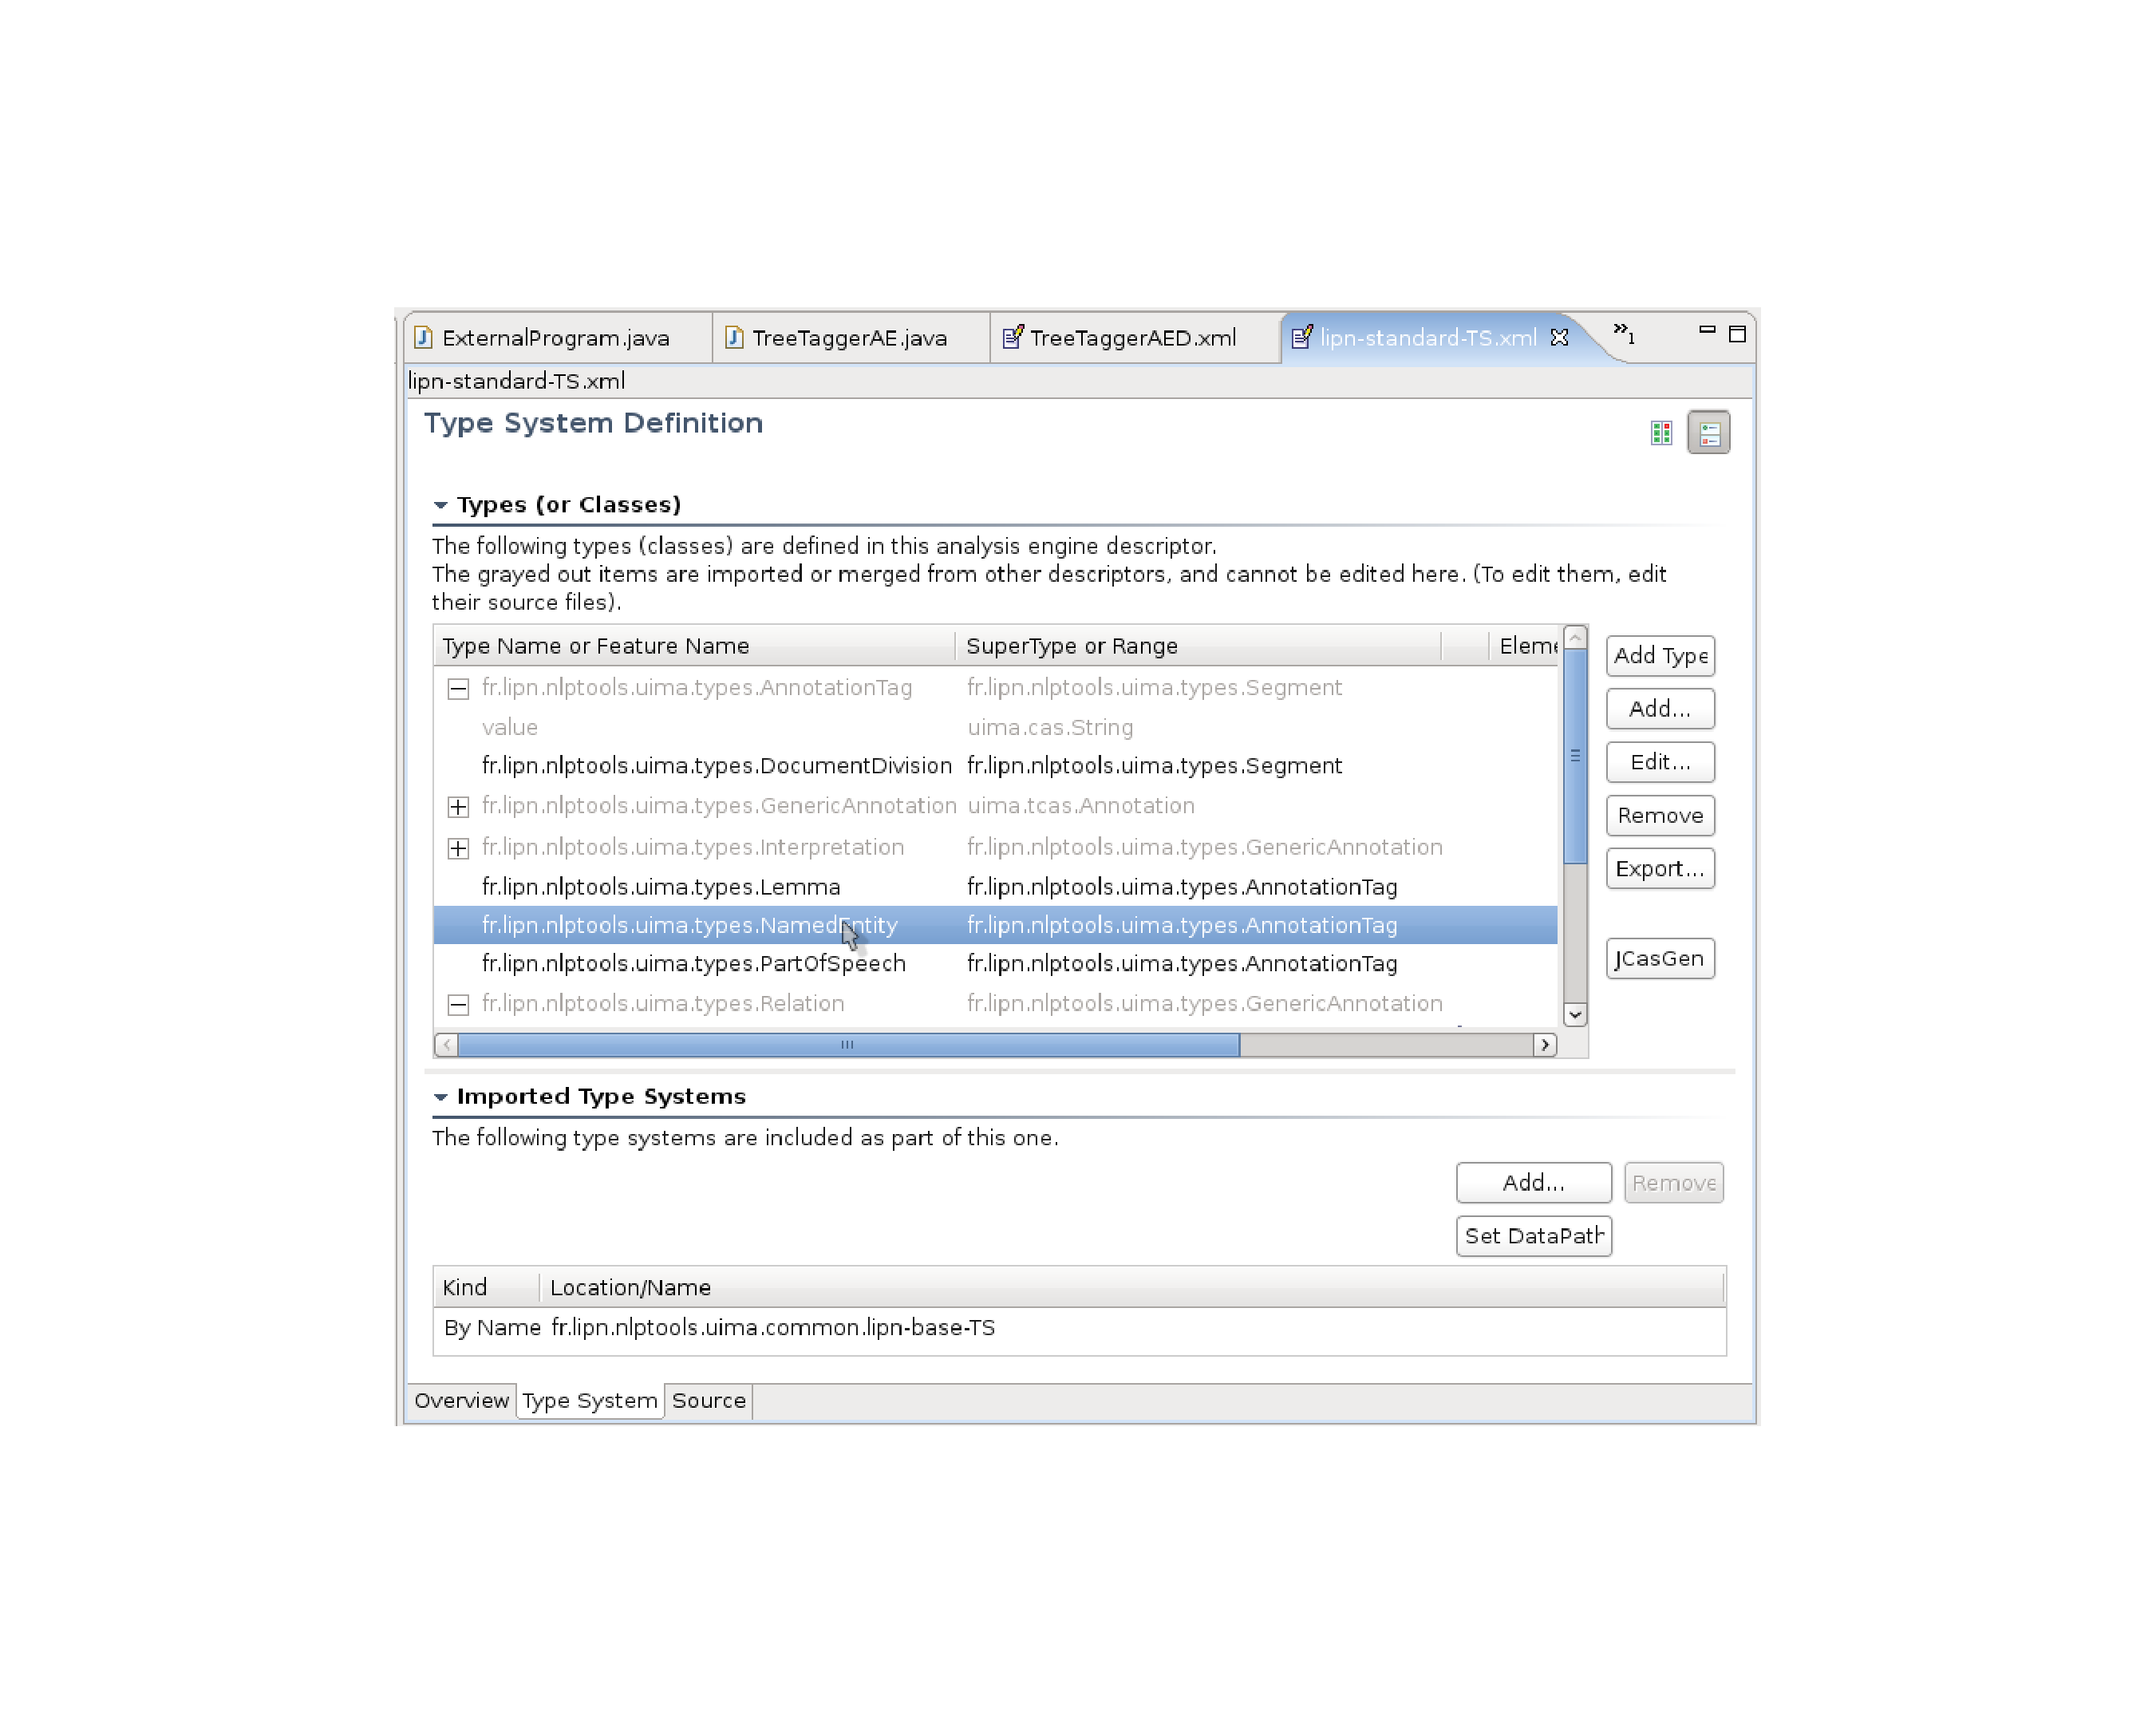
\includegraphics{capture_TS.eps}}

}

\subsection{Descripteur d'AE (Eclipse)}
\frame[plain]{
%\frametitle{le descripteur d'AE}

\vspace*{-.7cm}

\noindent\hspace*{-1.75cm}\scalebox{.32}[.32]{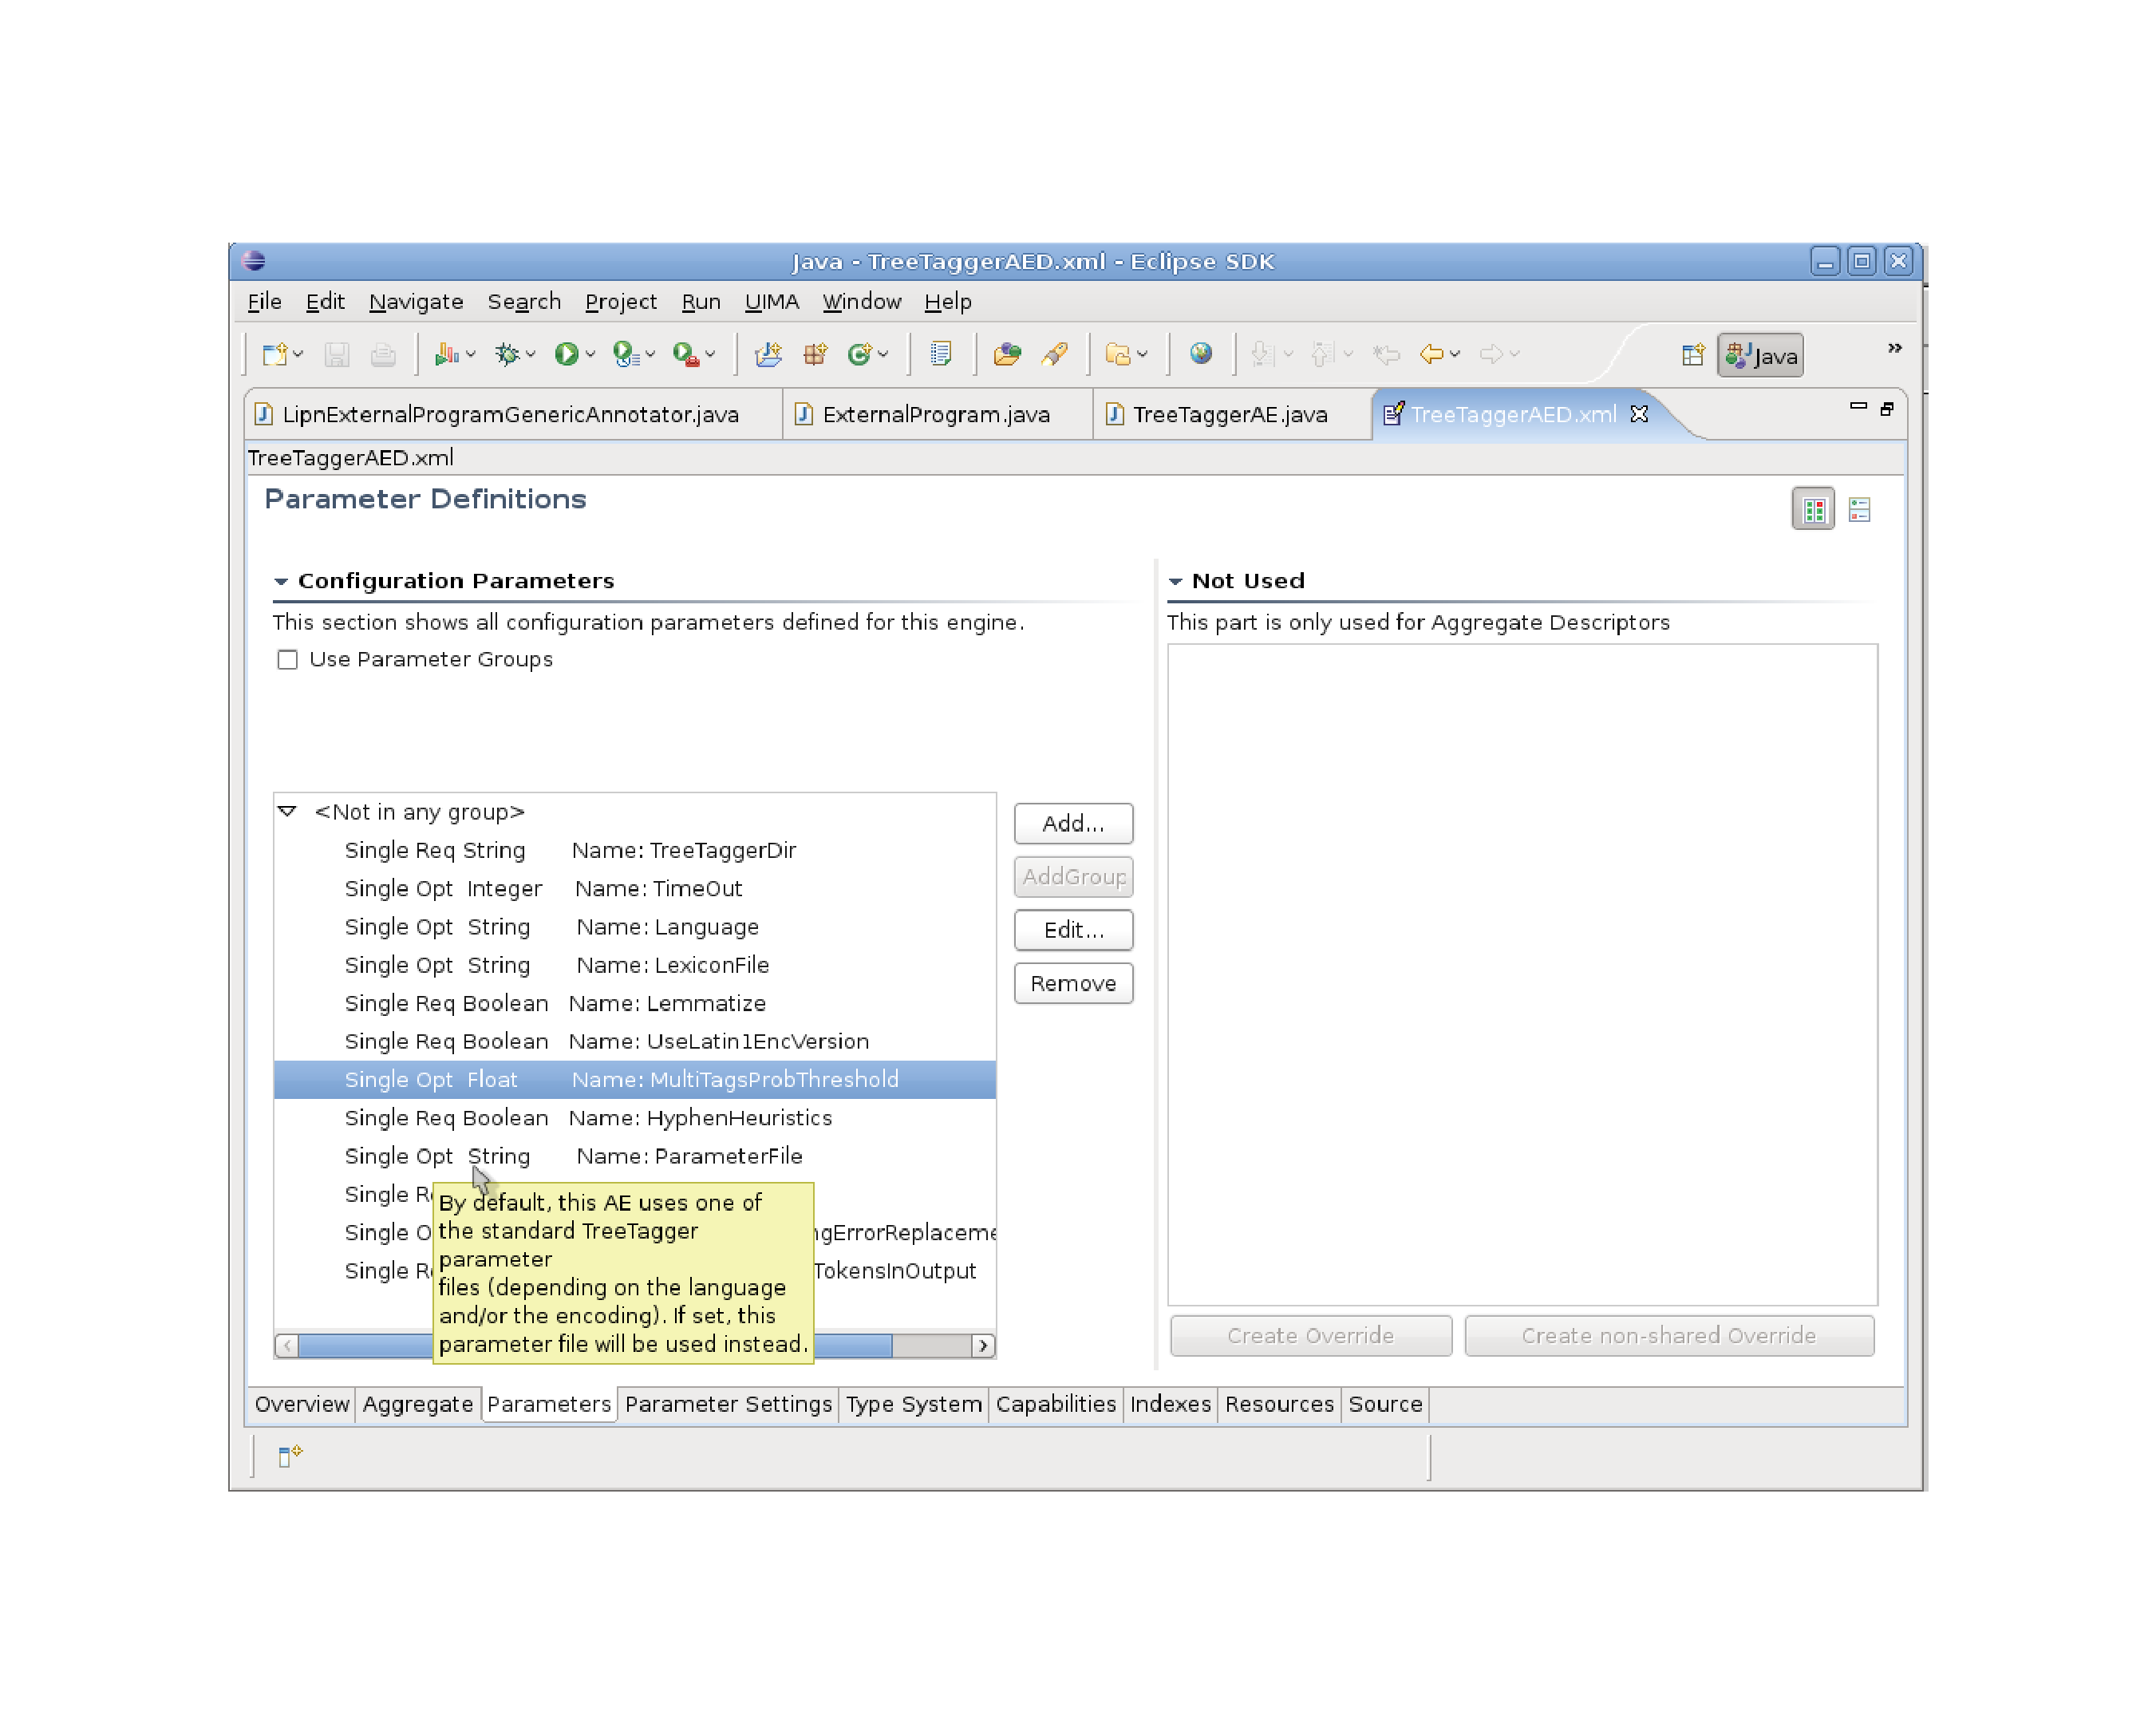
\includegraphics{capture_treetagger_AED.eps}}

}

\subsection{Configuration avec le CPE GUI}

\frame[plain]{
\frametitle{le CPE GUI}

\noindent\hspace*{-2.7cm}\scalebox{.36}[.33]{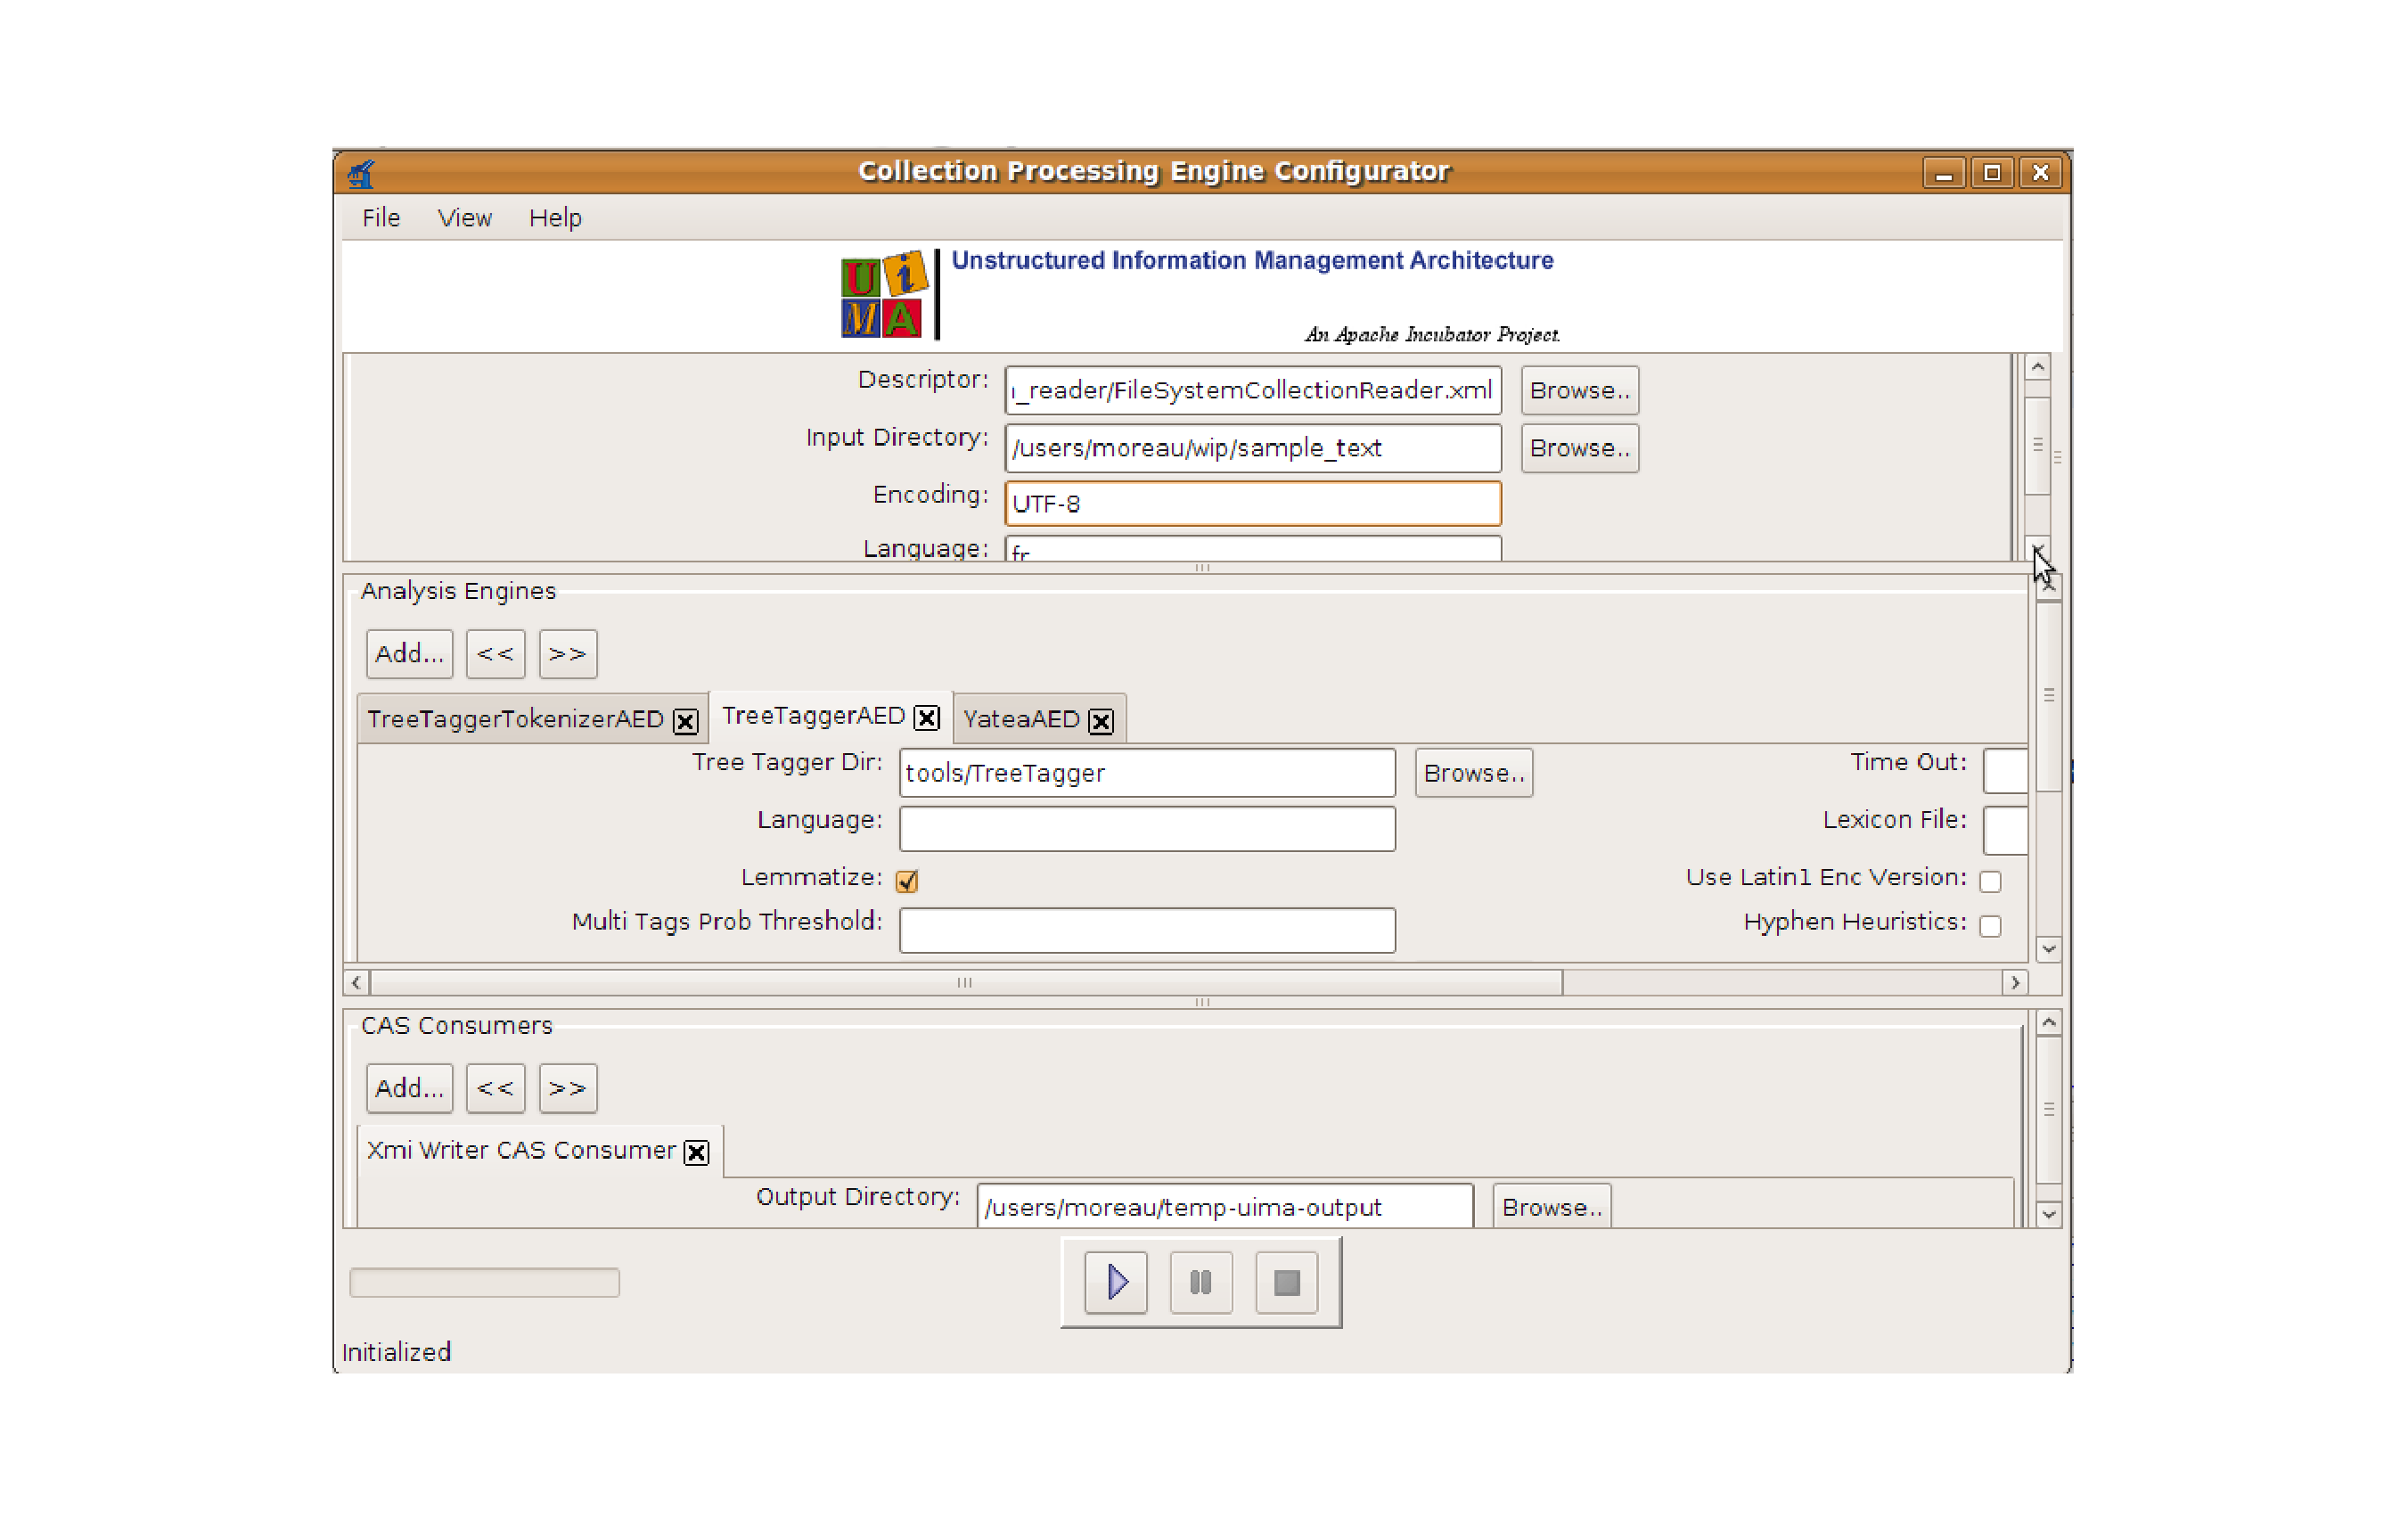
\includegraphics{capture_cpe_gui.eps}}

}


\subsection{Visualisation}

\frame[plain]{

\vspace*{.2cm}

%\noindent\begin{center}
\noindent\hspace*{-.35cm}\scalebox{.37}[.37]{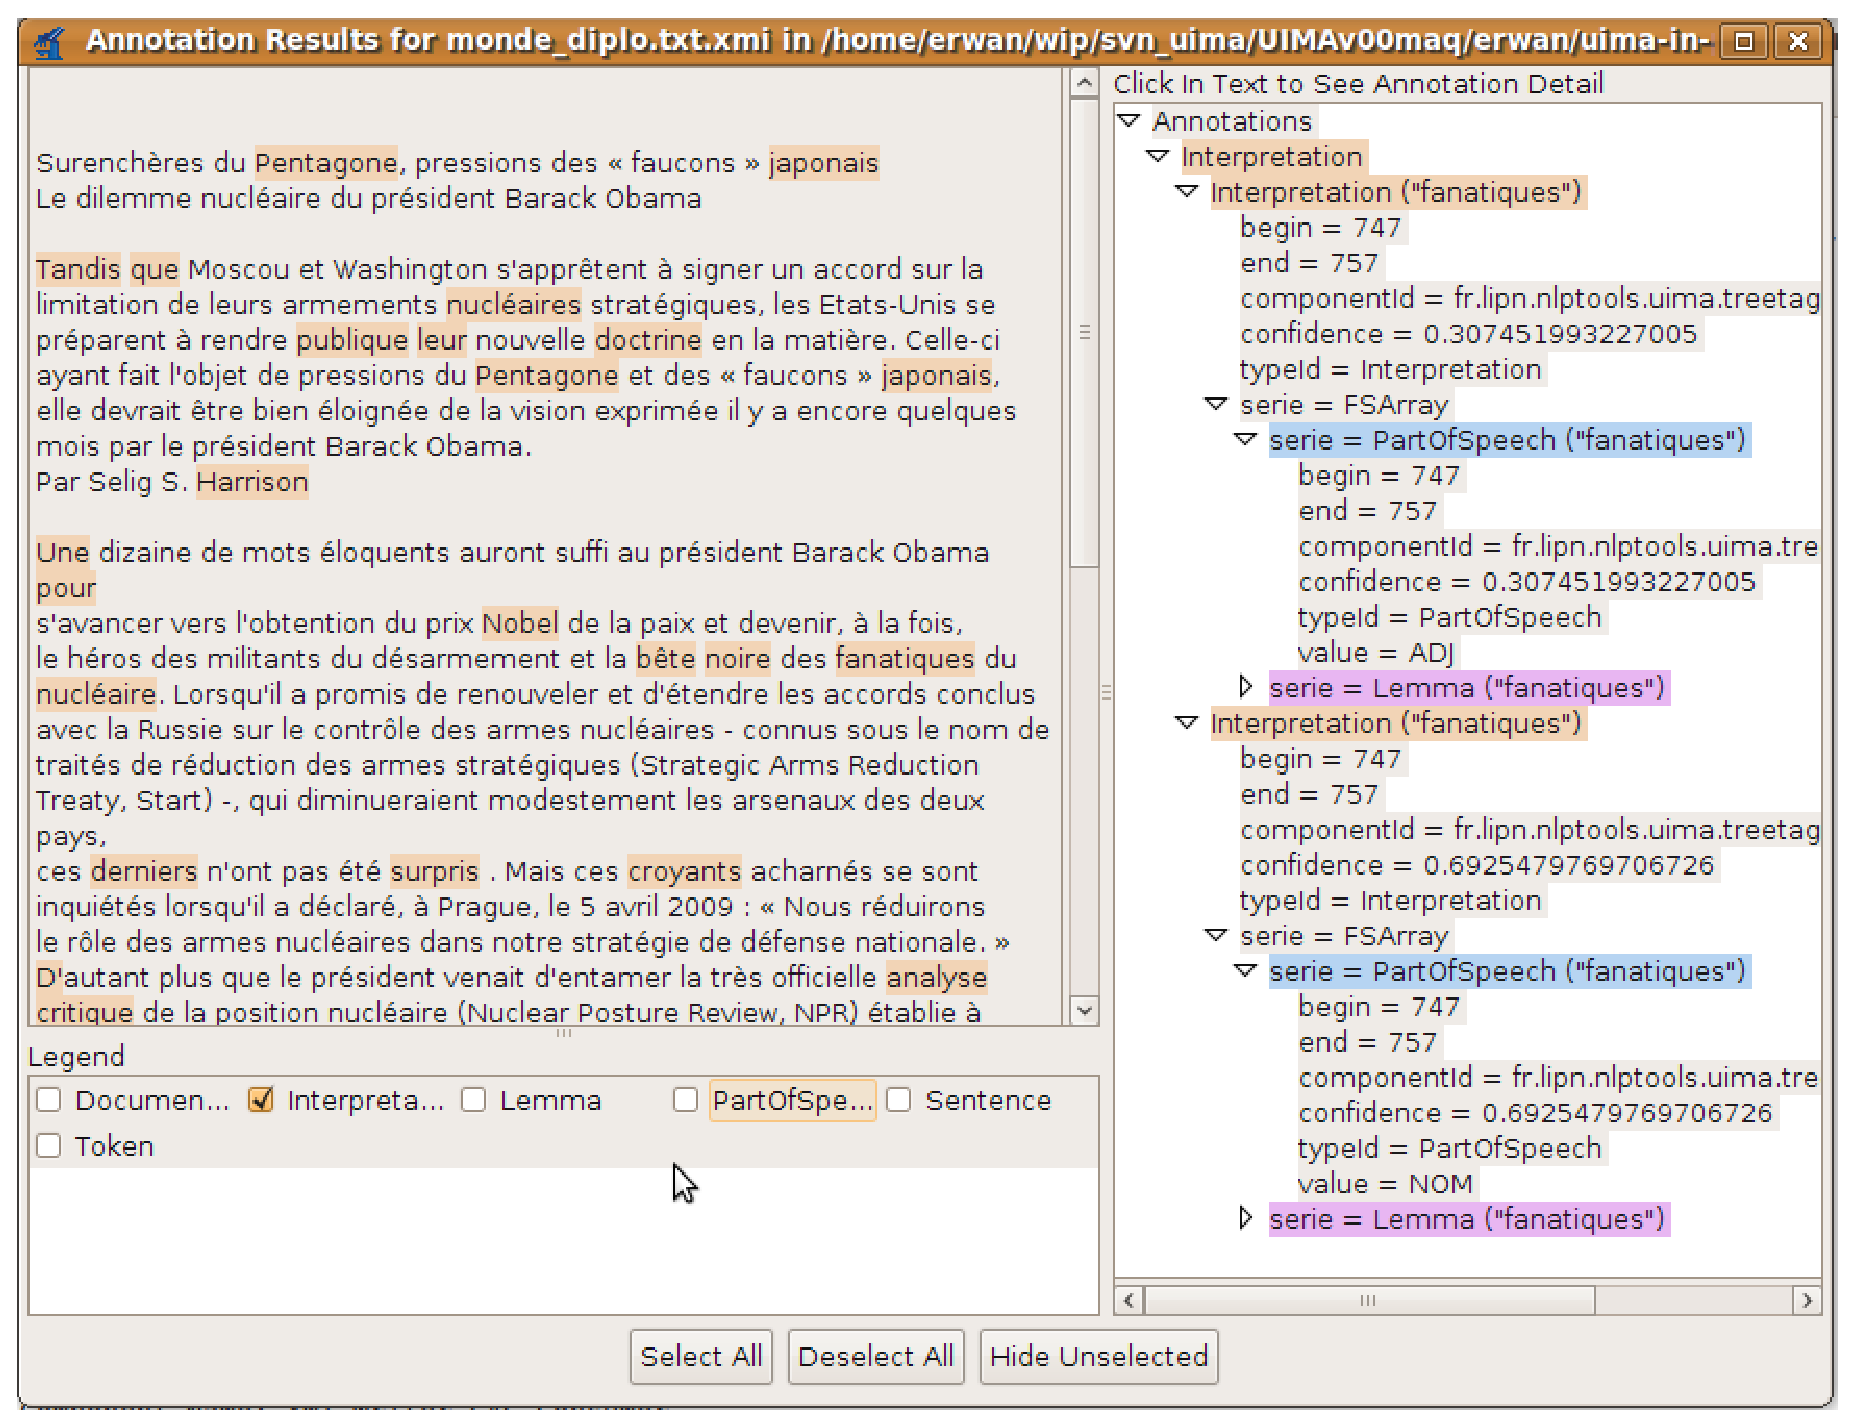
\includegraphics{capture_viewer_expl_interpretations.eps}}
%\end{center}

}


\section{Conclusion et perspectives}


%documentation

\subsection{Perspectives}

\frame{

\frametitle{Idées de composants futurs}

\begin{itemize}
\item Composants :
\begin{itemize}
\item Étiqueteur de termes
\item Segmenteur paramétrable
\item Analyse syntaxique (parser de Stanford,...)
\end{itemize}
\end{itemize}

\begin{itemize}
\item Intégration de composants UIMA extérieurs :
\begin{itemize}
\item Dunamis, outil graphique de paramétrage/visualisation (LINA)
\item Nombreux composants LINA : lecture de pdf, identifieur de langue, extraction de termes, etc.
\item OpenNLP Wrapper : intégration des composants OpenNLP
\end{itemize}
\end{itemize}
}

\subsection{Synthèse}


\frame{
\frametitle{Synthèse}

\begin{itemize}
\item Contre : nombreux inconvénients !
\begin{itemize}
\item Temps d'apprentissage/adaptation
\begin{itemize}
%\item compréhension de mécanismes inhabituels
\item problèmes fréquents de chemin/CLASSPATH
\end{itemize}
\item Cadre contraignant
\begin{itemize}
\item nécessité de se documenter souvent
\item tests plus laborieux
\end{itemize}
\end{itemize}
\item Pour : bénéfices à moyen/long terme
\begin{itemize}
\item Combinaisons complexes de composants
\item Simplifier le remplacement d'un composant par un autre 
\end{itemize}
\item[$\Rightarrow$] {\bf Utilité proportionnelle au niveau d'analyse}
\begin{itemize}
\item Plus il y a de phases antérieures, plus il est important :
\begin{itemize}
\item d'avoir des composants fiables aux niveaux inférieurs
\item de pouvoir paramétrer simplement ces niveaux inférieurs
\end{itemize}
\end{itemize}
\end{itemize}
}

\frame{
\frametitle{Stratégie de gestion des développements logiciels}

\begin{itemize}
\item Intérêts d'une politique de gestion logicielle
\begin{itemize}
\item Clarté des composants existants
\begin{itemize}
\item éviter les doublons
\item harmoniser les approches
\item éviter perte de temps à chercher bonne version, doc...
\end{itemize}
\item Maintenance facilitée
\begin{itemize}
\item centralisation des bugs/manques
\item trouver/corriger plus vite les problèmes
\end{itemize}
%\item Travail plus efficace à moyen terme
\end{itemize}
\item Moyens nécessaires :
\begin{itemize}
\item Dépôt centralisé (semi-)public
\item Identification des auteurs, versions, stabilité
\end{itemize}
\item Outils libres existants
\begin{itemize}
\item svn, maven,...
\item SourcesSup : plateforme de gestion de projets Enseignement Supérieur/ Recherche
\end{itemize}
\end{itemize}
%svn,maven, versions
}



\end{document}
